\documentclass[11pt]{beamer}
\usetheme{CambridgeUS}
\usepackage[utf8]{inputenc}
\usepackage{amsmath}
\usepackage{amsfonts}
\usepackage{amssymb}
\usepackage[
backend=biber,
style=alphabetic,
citestyle=authoryear
]{biblatex}

% Footnote without number
\newcommand\blfootnote[1]{%
  \begingroup
  \renewcommand\thefootnote{}\footnote{#1}%
  \addtocounter{footnote}{-1}%
  \endgroup
}

\addbibresource{stats.bib}
\title[Bioestatística II] %optional
{Distribuição Amostral da Média}

\subtitle{CGF2046 - Bioestatística II}

\author[da Silva, Ricardo] % (optional, for multiple authors)
{R. ~R. ~da Silva\inst{1}}

\institute[FCFRP] % (optional)
{
  \inst{1}%
  Departamento de Ciências BioMoleculares\\
  Faculdade de Ciências Farmacêuticas

}

\date{\today} % (optional)

\titlegraphic{
\includegraphics[width=5.8cm]{figs/logo_final}} 

\begin{document}

%\begin{frame}
%\titlepage
%\end{frame}

%\begin{frame}
%\tableofcontents
%\end{frame}

\begin{frame}
\titlepage
\end{frame}

\begin{frame}
\label{contents}
\frametitle{Sumário}
\tableofcontents
\end{frame}

\setbeamercovered{transparent}
\begin{frame}
\frametitle{Objetivos de Aprendizado}
  Depois de assitir essa aula e fazer as atividades complementares, você será capaz de:
  \\~\\
  \begin{itemize}
  \uncover<1->{\item
    Explicar como uma distribuição de médias amostrais é criada;}
  \uncover<2->{\item
    Explicar como uma amostra aleatória é obtida;}
  \uncover<3->{\item
    Determinar a média, o desvio padrão e a forma de uma distribuição de médias amostrais;}
   \uncover<4->{\item
    Explicar qual é o erro padrão das medidas médias;}
   \uncover<5->{\item
    Explicar o teorema central do limite e por que ele é importante;}
   \uncover<6->{\item
    Explicar a lei dos grandes números;}
   \uncover<7->{\item
    Calcular a z para uma média amostral;}
   \uncover<8->{\item Usar z para uma média amostral e uma tabela de probabilidades para distribuição normal para determinar a probabilidade de uma dada média amostral ocorrer;}
  \end{itemize}
\end{frame}

\section{Conceitos básicos de inferência}
\setbeamercovered{transparent}
\begin{frame}
\frametitle{Definições}
  Conceitos fundamentais
  \\~\\
  \begin{itemize}
  \uncover<1->{\item
    \textbf{População}: Conjunto de todos os elementos sob investigação.}
  \uncover<2->{\item
    \textbf{Amostra}: Subconjunto da população.}
  \uncover<3->{\item
    \textbf{Variável} de interesse: característica a ser observada em
    cada indivíduo da amostra.}
  \end{itemize}
\end{frame}

\setbeamercovered{transparent}
\begin{frame}
\frametitle{Variável aleatória}

\textbf{Definição}

\begin{itemize}
\item
  \textbf{Variável aleatória} - Descrição numérica do resultado de um
  fenômeno aleatório.
\end{itemize}

\textbf{Notação}

\begin{itemize}
\item
  \(X\) denota a variável aleatória.
\item
  \(x\) denota os valores realizados da v.a.
\item
  Probabilidade de \(X\) assumir o valor \(x\) é denotada \(P(X = x)\).
\end{itemize}

\textbf{Exemplo}

\begin{itemize}
\item
  X: Número de alunos em uma sala de aula.
\item
  Uma possível realização \(x = 50\).
\end{itemize}
\end{frame}

\setbeamercovered{transparent}
\begin{frame}
\frametitle{Parâmetro e Estimador}

\textbf{População} \(\rightarrow\) \textbf{censo} \(\rightarrow\)
\textbf{parâmetro}

\emph{Uma medida numérica que descreve alguma característica da
\textbf{população}, usualmente representada por letras gregas:
\(\theta\), \(\mu\), \(\sigma\), \(\ldots\)}

Exemplo: média populacional = \(\mu\)

\vspace{1em}
\hrule
\vspace{1em}

\textbf{População} \(\rightarrow\) \textbf{amostra} \(\rightarrow\)
\textbf{Estimador}

\emph{Uma medida numérica que descreve alguma característica da
\textbf{amostra}, usualmente denotada pela letra grega do respectivo
parâmetro com um acento circunflexo: \(\hat\theta\), \(\hat\mu\),
\(\hat\sigma\), \(\ldots\), ou por letras do alfabeto comum: \(\bar x\),
\(s\), \(\ldots\)}

Exemplo: média amostral = \(\bar{x}\)
\end{frame}

\setbeamercovered{transparent}
\begin{frame}
\frametitle{Estimador}

\textbf{Observação:}

\begin{enumerate}
\def\labelenumi{\arabic{enumi}.}

\item
  O valor assumido pelo estimador pontual é chamado de
  \textbf{estimativa
  pontual},\[\hat{\theta} = T(\mathbf{X}) = T(X_1, \ldots, X_n) = t\] ou
  seja, o estimador é uma \textbf{função} da amostra, e a estimativa é o
  \textbf{valor observado} de um estimador (um número) de uma amostra
  particular.
\end{enumerate}
\end{frame}

\setbeamercovered{transparent}
\begin{frame}
\frametitle{Média de dados brutos}

Divide-se a soma de todos os dados pelo número total deles:

\[
\bar{x}_{obs} = \frac{x_1 + x_2 + \cdots + x_n}{n} = \frac{\sum_{i=1}^n
x_i}{n}.
\]
\begin{center}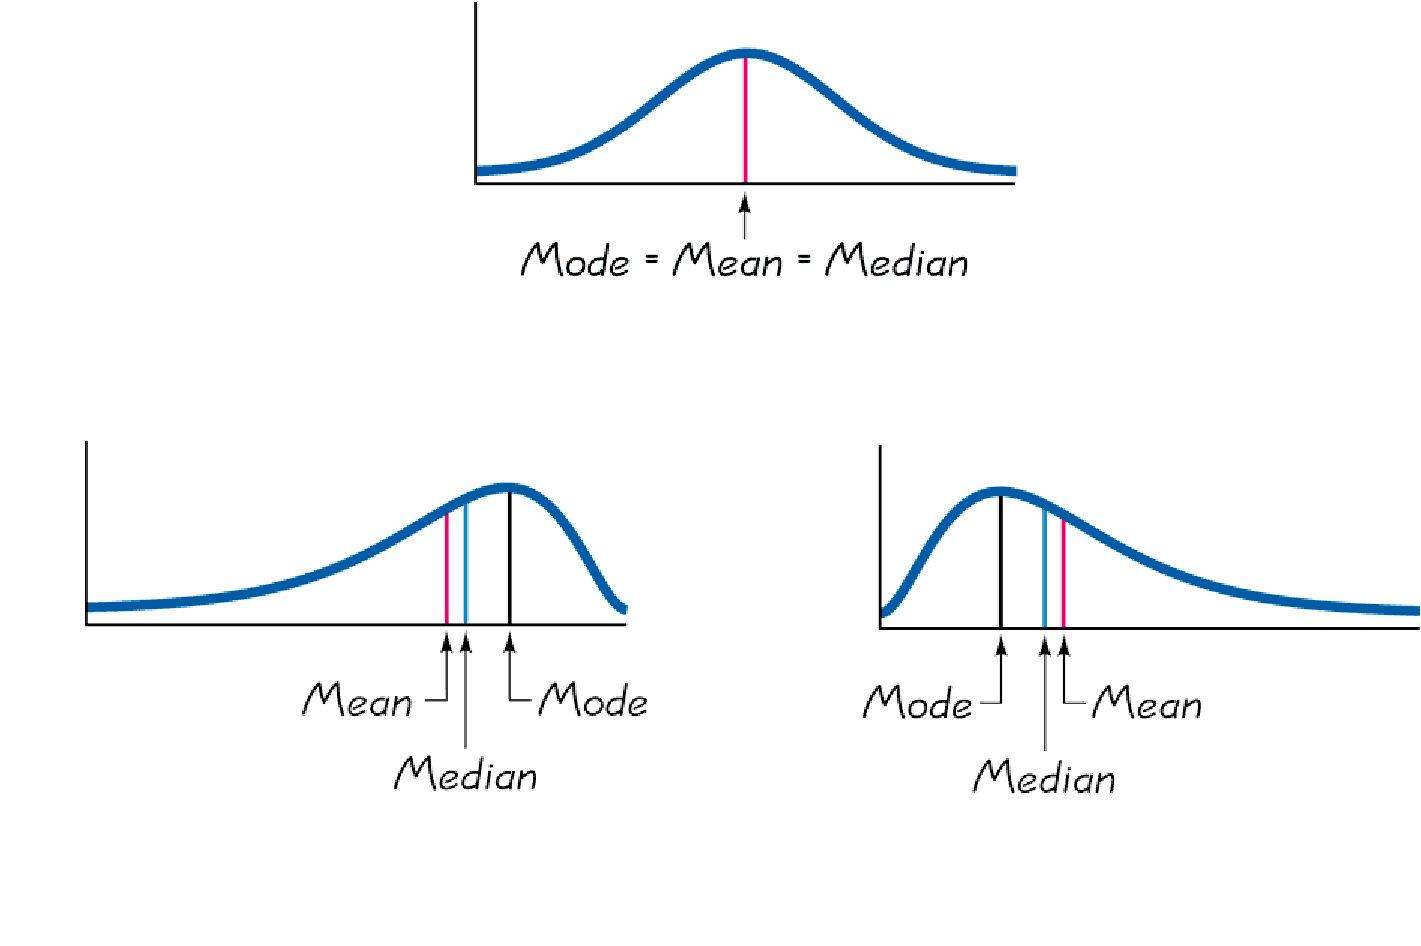
\includegraphics[width=0.8\linewidth]{figs/medidas-crop} \end{center}
\end{frame}

\setbeamercovered{transparent}
\begin{frame}
\frametitle{Variância e desvio-padrão de um conjunto de dados}

Uma alternativa melhor é usar a \textbf{soma dos quadrados dos desvios},
que dá origem à \textbf{variância} de um conjunto de dados \[
var_{obs} = \frac{1}{n}\sum_{i=1}^n (x_i - \bar{x}_{obs})^2
\] Para manter a mesma unidade de medida dos dados originais, definimos
o \textbf{desvio padrão} como \[
dp_{obs} = \sqrt{var_{obs}}
\] Uma expressão alternativa da variância (mais fácil de calcular) é \[
var_{obs} = \frac{1}{n}\sum_{i=1}^n x_i^2 - \bar{x}_{obs}^2
\]
\end{frame}


\section{Distribuição Amostral}
\setbeamercovered{transparent}
\begin{frame}
\frametitle{Intuição para distribuições amostrais}
Uma distribuição de médias amostrais é a população de todas as médias amostrais aleatórias possíveis para um estudo realizado com um determinado tamanho de amostra.\\~\\
População exemplo de quatro valores: \[10, 12, 14, 16\]

\end{frame}

\setbeamercovered{transparent}
\begin{frame}
\frametitle{Exemplo}
Distribuição de médias amostrais para a população de quatro valores e um tamanho de amostra de 2
\begin{center}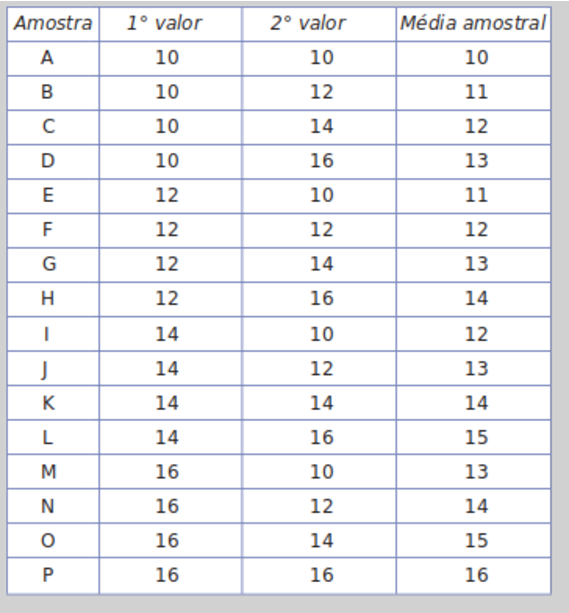
\includegraphics[width=0.5\linewidth]{figs/chap5tab5.2} \end{center}
\end{frame}

\setbeamercovered{transparent}
\begin{frame}
\frametitle{Parâmetros \textit{vs} Estimativas}
A média da população é dada por:
\[\mu=\frac{1}{N}\sum_{i=1}^Nx_i=\frac{52}{4}=13\]
A média da distribuição das médias amostrais, as 16 médias amostrais na última coluna da tabela anterior é dada por
\[\bar{X}=\frac{1}{N}\sum_{i=1}^N\bar{x}_i=\frac{208}{16}=13\]

\end{frame}

\setbeamercovered{transparent}
\begin{frame}
\frametitle{Distribuição das médias}
O fato de a média da distribuição das médias amostrais ser sempre igual à média da população original mostra que quando os pesquisadores selecionam aleatoriamente uma amostra para usar em seus estudo, selecionar uma amostra que tenha a mesma média da população, ou uma média próxima a ela, é bastante comum.
\begin{center}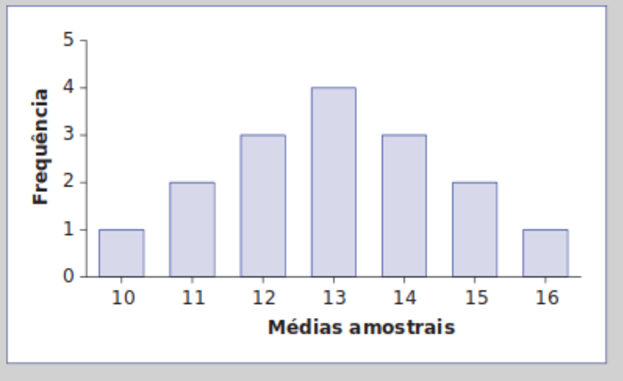
\includegraphics[width=0.6\linewidth]{figs/chap5fig5.1} \end{center}

\end{frame}

\setbeamercovered{transparent}
\begin{frame}
\frametitle{Desvios padrão populacional e amostral}
A variância da população pode ser obtida por
\[\sigma^2 = \frac{1}{n}\sum_{i=1}^n x_i^2 - \mu^2=\frac{1}{4}696-169=5\]
E o desvio padrão
\[\sigma= \sqrt{\sigma^2} = 2.24\]
A variância da distribuição amostral pode ser obtida por
\[Var(X) = \frac{1}{n}\sum_{i=1}^n \bar{x}_i^2 - \bar{X}^2=\frac{1}{16}2744-169=2.5\]
E o desvio padrão
\[DP = \sqrt{Var(X)} = 1.58\]
\end{frame}

\setbeamercovered{transparent}
\begin{frame}
\frametitle{Erro padrão da média}
O erro padrão de um estimador é o desvio padrão de sua distribuição amostral. Para o estimador da média, temos o erro padrão da média
\[\sigma_{\bar{X}} = SEM = \frac{\sigma}{\sqrt{N}}\]
onde \(\sigma\) representa o devio padrão populacional e \(N\) o tamanho da amostra.
Para o nosso exemplo, o erro padrão da média pode ser obtido por
\[SEM = \frac{\sigma}{\sqrt{N}} = \frac{2.24}{\sqrt{2}}=1.58\]

\end{frame}

\setbeamercovered{transparent}
\begin{frame}
\frametitle{Observações do experimento númerico}
Observamos empiricamente, que:
\begin{itemize}
\item A média da distribuição das médias amostrais é igual a média populacional, \(\mu\);
\item O desvio padrão é sempre igual ao SEM, \(\sigma/N\);
\item O gráfico da distribuição da amostral tem distribuição aproximadamente normal (ou seja, em forma de sino).
\end{itemize}

\end{frame}


\setbeamercovered{transparent}
\begin{frame}
\frametitle{Outros experimentos númericos}
\begin{center}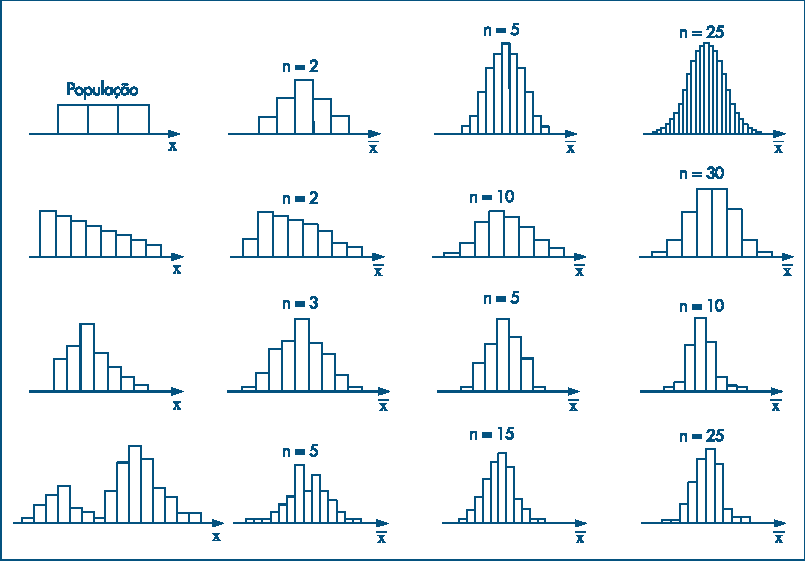
\includegraphics[width=0.9\linewidth]{figs/func2}\end{center}
\end{frame}

\setbeamercovered{transparent}
\begin{frame}
\frametitle{Distribuições amostrais}

\begin{block}{Distribuições amostrais}

A distribuição de probabilidade de uma estatística
\(Y = T(x_1, x_2, \ldots, x_n)\) é denominada de \textbf{distribuição
amostral} de \(Y\). Assim, uma estatística também é uma variável
aleatória, pois seus valores mudam conforme a amostra aleatória.
\end{block}

\begin{block}{}
\textbf{Exemplo}: duas estatísticas comumente utilizadas para o resumo
de uma amostra aleatória são a \textbf{média amostral} \(\bar{x}\), e a
\textbf{proporção amostral} \(\hat{p}\). Cada uma delas também possui
uma distribuição amostral.
\end{block}
\end{frame}

\setbeamercovered{transparent}
\begin{frame}
\frametitle{Distribuição amostral da média}

Através do estudo da distribuição da média amostral chegamos em um dos
resultados mais importantes da inferência estatística.

\begin{block}{Distribuição amostral da média}

\begin{itemize}
\item
  \(\text{E}(\bar{X}) = \mu_{\bar{X}} = \mu\)
\item
  \(\text{Var}(\bar{X}) = \sigma^2_{\bar{X}} = \sigma^2/n\)
\end{itemize}

Portanto, se \[X \sim \text{N}(\mu, \sigma^2) \quad \text{então} \quad
\bar{X} \sim \text{N}(\mu_{\bar{X}}, \sigma^2_{\bar{x}})\] mas, como
\[\mu_{\bar{X}} = \mu \quad \text{e} \quad \sigma^2_{\bar{X}} =
\sigma^2/n\] então, a \textbf{distribuição amostral} da média amostral
\(\bar{X}\) é
\[\bar{X} \sim \text{N}\left(\mu, \frac{\sigma^2}{n} \right)\]
\end{block}
\end{frame}

\setbeamercovered{transparent}
\begin{frame}
\frametitle{Distribuição amostral da média}

Pode-se mostrar que, para amostras suficientemente grandes, \textbf{a
média amostral \(\bar{X}\) converge para o verdadeiro valor da média
populacional \(\mu\)} (é um \textbf{estimador não viesado} de \(\mu\)).

Além disso, a variância das médias amostrais \(\sigma^2_{\bar{X}}\)
tende a diminuir conforme \(n \rightarrow \infty\) (é um estimador
\textbf{consistente}).

Estes resultados sugerem que, quando o tamanho da amostra aumenta,

\begin{center}
\underline{independente do formato da distribuição da população
original},
\end{center}

\textbf{a distribuição amostral de \(\bar{X}\) aproxima-se cada vez mais
de uma distribuição Normal}, um resultado fundamental na teoria de
probabilidade conhecido como \textbf{Teorema Central do Limite}.
\end{frame}


% adicionar figura 7.15
\setbeamercovered{transparent}
\begin{frame}
\frametitle{Distribuição amostral da média}

\begin{block}{Teorema Central do Limite (TCL)}

Para amostras aleatórias simples \((X_1, X_2, \ldots, X_n)\), retiradas
de uma população com média \(\mu\) e variância \(\sigma^2\), a
distribuição amostral da média \(\bar{X}\), terá forma dada por \[
Z = \frac{\bar{X} - \mu}{\sigma/\sqrt{n}}
\] no limite quando \(n \to \infty\), onde \(Z \sim \text{N}(0,1)\).

\end{block}

O teorema garante que para \textit{n} grande a distribuição da média amostral, devidamente padronizada, se comporta segundo um modelo Normal com média 0 e variância 1.

\end{frame}

\setbeamercovered{transparent}
\begin{frame}
\frametitle{Exemplo 7.14}
Suponha que a aceitação de um lote de 1000 peças ocorra apenas, se o comprimento médio de 10 peças, retiradas aleatoriamente do lote, estiver entre 5 e 10 \(cm\). Sabe-se que o comprimento das peças é uma variável aleatória com distribuição Normal de média 7.5 e variância 20 \(cm^2\). Qual é a probabilidade de aceitação de um dado lote?
\vspace{1in}
\vspace{1in}

\end{frame}

\begin{frame}
\frametitle{Distribuição Normal}

%\begin{center}\includegraphics[width=0.8\linewidth]{../figures/tabela_Z_01} \end{center}
\end{frame}


\setbeamercovered{transparent}
\begin{frame}
\frametitle{Exemplo 7.15}
Uma variável aleatória X assume valores 3, 6 e 8 com, respectivamente, probabilidades 0.4; 0.3 e 0.3. Uma amostra com 40 observações é sorteada. A variável X não tem distribuição Normal e obtemos \(\mu=5.4\) e \(\sigma^2=4.44\). Calcule a probabilidade da média amostral superar o valor 5.
\vspace{1in}
\vspace{1in}

\end{frame}

\end{document}